%%%%%%%%%%%%%%%%%% DOCUMENT SETUP %%%%%%%%%%%%%%%%%%

% Required IEEE parameters
\documentclass[letterpaper, 10pt, conference]{ieeeconf} % set document type
%\documentclass[10pt,journal,compsoc]{IEEEtran}
\IEEEoverridecommandlockouts                              % for \thanks command
%\overrideIEEEmargins                             % use for \addtolength to normalize column lengths


% Packages
\usepackage{graphicx} % allows additional graphics formats
  \graphicspath{ {./images/} }
\usepackage{amsmath}   % assumes amsmath package installed
  \allowdisplaybreaks[1] % allow eqnarrays to break across pages
\usepackage{amssymb}   % assumes amsmath package installed 
\usepackage{url}       % format hyperlinks correctly
\usepackage{rotating}  % allow portrait figures and tables
\usepackage{subfigure} % allow matrices of figures
\usepackage{float}     % allows H option on floats to force here placement
\usepackage{multirow}  % allows merging of rows in tables
\usepackage{tabularx}  % allows fixed width tables
\usepackage{ctable}    % modifies \hline for use in table
\usepackage{bm}        % allow bold fonts in equations
\usepackage{wrapfig}   % allow text wrapping round figures
\usepackage{stfloats}  % control placement of floats
\usepackage[backend=biber,style=ieee,maxbibnames=3,bibencoding=utf8]{biblatex}   % allow bibliography control 
  \addbibresource{journal_abbreviations.bib}
  \addbibresource{references.bib}
\usepackage{siunitx}
\usepackage{placeins}
\usepackage[ruled,vlined]{algorithm2e}
\include{pythonlisting}
% Custom commands
\newcommand{\matlab}{\emph{\sc{Matlab}}}
\newcommand{\maple}{\emph{\sc{Maple}}}
\newcommand{\simulink}{\emph{\sc{Simulink}}}
\newcommand{\dc}{d.c.}
\newcommand{\ac}{a.c.}
\newcommand{\rms}{RMS}
\newcommand{\wgn}{{\tt wgn}}
\newcommand{\sus}[1]{$^{\mbox{\scriptsize #1}}$}
\newcommand{\sub}[1]{$_{\mbox{\scriptsize #1}}$}
\newcommand{\chap}[1]{Chapter~\ref{#1}}
\newcommand{\sect}[1]{Section~\ref{#1}}
\newcommand{\fig}[1]{Fig.~\ref{#1}}
\newcommand{\tab}[1]{Table~\ref{#1}}
\newcommand{\equ}[1]{(\ref{#1})}
\newcommand{\appx}[1]{Appendix~\ref{#1}}
\newcommand{\degree}{\ensuremath{^\circ}}
\newcommand{\Vrms}{V\sub{\rms}}
\newcommand{\Vpp}{V\sub{pp}}
\newcommand{\otoprule}{\midrule[\heavyrulewidth]}         
\newcolumntype{Z}{>{\centering\arraybackslash}X}  % tabularx centered columns 
\newcommand\norm[1]{\left\lVert#1\right\rVert}

%\usepackage{setspace}
\usepackage[noend]{algpseudocode}

\usepackage{flushend}
% Adjust figure spacing to get more text onto each page
\setlength{\abovecaptionskip}{2pt}
\setlength{\belowcaptionskip}{2pt}
\setlength{\dbltextfloatsep}{8pt}
\setlength{\dblfloatsep}{3pt}
\setlength{\floatsep}{3pt}
\setlength{\textfloatsep}{2pt}
%\addtolength{\skip\footins}{-10pt}


%%%%%%%%%%%%%%%%%% TITLE AND FRONT MATTER %%%%%%%%%%%%%%%%%%

% Title
\title{\LARGE \bf An efficient deep learning model for intrusion classification and prediction in 5G and IoT networks}

% Authors and affiliations 
\author{\IEEEauthorblockA{Shahadate Rezvy, Yuan Luo, Miltos Petridis, Aboubaker Lasebae}\\ School of Science \& Technology\\
\IEEEauthorblockA{Middlesex University London, UK\\
Email: \{s.rezvy, y.luo, m.petridis, a.lasebae\}@mdx.ac.uk}
\and
\IEEEauthorblockB{Tahmina Zebin }  \\  School of Computer Science \& Engineering\\
\IEEEauthorblockB{University of Westminster, UK\\
Email: t.zebin@westminster.ac.uk}
}



% Setup document 
\begin{document}
\maketitle
\thispagestyle{empty} % stop page numbers
\pagestyle{empty}


%%%%%%%%%%%%%%%%%% ABSTRACT %%%%%%%%%%%%%%%%%%
\begin{abstract}
A Network Intrusion Detection System  is a critical component of every internet-connected system due to likely attacks from both external and internal sources. Such Security systems are used to detect network born attacks such as flooding, denial of service attacks, malware, and twin-evil intruders that are operating within the system. Neural networks have become an increasingly popular
solution for network intrusion detection. Their capability of learning complex patterns and behaviors make them a suitable solution for differentiating between normal traffic and network attacks. In this paper, we have applied a deep autoencoded dense neural network algorithm for detecting intrusion or attacks in 5G and IoT network. We evaluated the algorithm with the benchmark Aegean Wi-Fi Intrusion dataset. Our  results  showed  an  excellent  performance  with  an overall  detection  accuracy  of  99.9\%  for  Flooding,  Impersonation and  Injection type  of attacks. We also presented a comparison with recent approaches used in literature which showed a substantial improvement in terms of accuracy and speed of detection with the proposed algorithm.

\end{abstract}

% Note that keywords are not normally used for peerreview papers.
\begin{keywords}
computer network security, deep learning, intrusion detection system, autoencoder, dense neural network.
\end{keywords}

% make the title area






%http://cis.csuohio.edu/~sschung/CIS601/Arida_ResearchProposal_Example.pdf

%%%%%%%%%%%%%%%%%% INTRODUCTION %%%%%%%%%%%%%%%%%%
\section{Introduction} \label{sec:introduction}

%Over the past few decades, the Internet has penetrated all aspects of our lives. 

 Cyber-attacks have increased by an alarming rate as the Internet of Things (IoT) are widely used now-a-days to provide e-commerce, to give online access to health-care, communication and billing systems. Experts predict that by 2020, wireless network traffic is anticipated to account for two-thirds of total Internet traffic to be generated by 50 billion  Wi-Fi and cellular connected devices \cite{Shone2018}. As technology becomes more and more integrated, security of these systems over wireless networks is becoming more important. Any hacks in banking systems, healthcare systems and many Internet of Things (IoT) devices could cause huge monetary losses every year and loss of services at crucial times.  This drove to an increase in research for more secured online systems specifically in the intrusion detection systems \cite{kolias2017, aminanto2018deep,alotaibi2016majority}. With the majority of internet traffic occurring over wireless networks, and the domain is constantly updating with 5G and IoT technologies, there are likely many gaps in the security of these networks that can be exploited through intrusion attempts. Therefore, wireless intrusion detection
systems are rapidly being developed in order to counter these potentially malicious behaviors.  Recently, deep learning based methods have been successfully implemented in Network Intrusion Detection Systems (NIDS) applications. Deep learning can substitute for manually designed feature extraction to create more secure firewall or intrusion detector \cite{ref:survey18}. Modern intrusion detection systems that uses deep learning (hierarchical learning) approaches for learning traffic data representations is meant to effectively detect or prevent various kinds of intrusion in wired or wireless networks.
 
 In this work, we have proposed a data mining based hybrid intrusion detection system for distinguishing normal and intrusive events from the AWID dataset \cite{AWID}. We focused on exploring low latency models  while  maintaining  high  accuracy  by  proposing a deep auto-encoded dense neural network (DNN) framework for effective intrusion detection. The NIDS using deep learning did alleviate the need of feature selection or feature engineering during the detection process.  In our design, the autoencoder facilitated an unsupervised pre-tarining on the data to provide compressed and less noisy representation of the input space, while the final dense neural network functioned as the supervised classifier for our experimental intrusion detection scenario.





% However, for the practitioner it is difficult to select the most suitable deep learning method for their application. 


 %rewrite this section once finished

The remainder of this paper is organized as follows. \sect{sec:methods} introduces the background literature in the recent development in intrusion detection systems using deep learning techniques, we then provide details on our parameter settings for the implemented model in section III. The performance of the developed model for attack classification is evaluated in section IV. We also compared the results with some recent deep learning techniques appeared in the literature using the same dataset. Finally, the paper is concluded in section V along with ideas for future work.



%%%%%%%%%%%%%%%%%% BACKGROUND %%%%%%%%%%%%%%%%%%
 \begin{figure*}
    \centering
  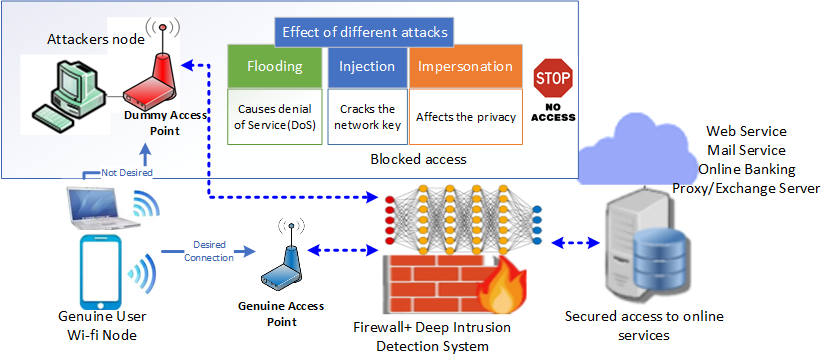
\includegraphics[width=0.755\textwidth]{Figures/NIDS.png}
%  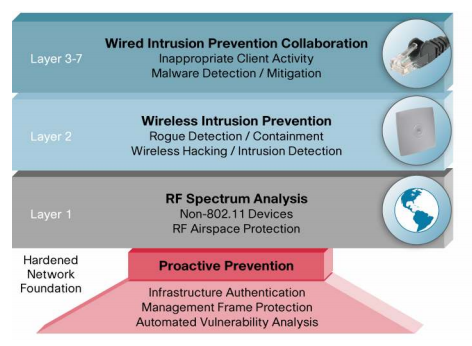
\includegraphics[width=0.75\textwidth]{Figures/WLAN_IDS.PNG}
    \caption{Illustration of the proposed network intrusion detection system(NIDS)}
    \label{fig:NIDS}
  \end{figure*}
  

%%%%%%%%%%%%%%%%%% METHODS %%%%%%%%%%%%%%%%%%
\section{Related Work} \label{sec:methods}
%     \begin{figure}
%       \centering
% %       \includegraphics[width=0.45\textwidth]{classifier_architecture.png}
%       \caption{Proposed deep neural network architecture for attack type classification.}
%       \label{fig:architecture}
%     \end{figure}
In recent years, machine learning has been widely applied to problems in detecting network attacks, particularly novel attacks.  Given the landscape of the Internet, machine learning can be applied to handle the massive amounts of traffic to determine what is malicious or benign. NIDS are classifiers that differentiate unauthorized or anomalous
traffic from authorized or normal traffic. \fig{fig:NIDS} shows an illustration of the proposed components for the NIDS implementation. In recent years, neural networks have become an increasingly popular solution for network intrusion detection systems (NIDS). Their capability of learning complex patterns and behaviors make them a suitable solution for differentiating between normal traffic and network attacks \cite{Yisroel2018}. One of the earliest work found in literature that used deep learning approach with Deep Belief Network (DBN) as a feature selector and Support Vector Machine (SVM) as a classifier were reported in \cite{salama2011}.

% https://www.ijcaonline.org/archives/volume180/number14/jayaswal-2018-ijca-916270.pdf
As traditional machine learning methods depend heavily on feature engineering, extracting features is often time-consuming and complex. Thus, it is impractical to detect attacks with traditional machine learning methods in real-time applications \cite{LIU2018}. 
%%%%%%%%%%%%%%%%%%%%%%%%%%%%%%%%%%%%%%%%%%%%%%%%%%%%%%%%%%%%%%%%%%%%  
  \begin{table*}[t]
\centering
\caption{ Broad attack types in the AWID dataset \cite{AWID,AWID_main} }
\label{table:KDD}
{\def\arraystretch{1.35}\tabcolsep=10pt
\begin{tabular}{p{2cm} p{9.5cm} p{3.5cm} }
\toprule
Broad attack type 	& Description of the attack &	Sub-categories in AWID 	\\
\otoprule


Flooding
 & {This category of attack is designed to cause an interruption or suspension of services of a specific host/server by flooding it with large quantities of useless traffic or external communication requests. When the Denial of Service (DoS) attack succeeds the server is not able to answer even to legitimate requests any more - this can be observed in numbers of ways: slow response of the server, slow network performance, unavailability of software or web page, inability to access data, website or other resources. } &	{deauthentication, authentication request, amok, probe request, probe response, beacon, cts, rts, power saving, disassociation, power} \\
Impersonation & {Impersonation takes the form of device cloning, address spoofing, unauthorized access, rogue base station (or rogue access point) and replay. For example, in an evil twin setup, the client(s) unknowingly connect to them under the pretext that they are connected to a genuine access point. Once a client is connected, an attacker eavesdrops on its communication to hijack client’s communication, re-direct clients to malicious websites, steal credentials of the clients connecting to it \cite{aminanto2017improving, Agarwal2018Evil_twin}. }	& {evil-twin, caffe-latte, hirte}\\

Injection 
 & {Attacker uses existing vulnerabilities in the applications to inject a code/string for execution that exceeds the allowed and expected input to the system requested, e.g.  inject a client-side script onto the webpage or an SQL database} &	{arp, fragmentation, chop chop}\\



\bottomrule
\end{tabular}}
\end{table*}
%    \begin{figure}
%     \centering
%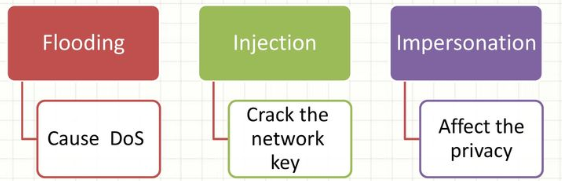
\includegraphics[width=0.49\textwidth]{Figures/attack_types.PNG}
%https://slideplayer.com/slide/13274380/
%https://resources.infosecinstitute.com/wireless-attacks-unleashed/#gref
%\caption{Effect of different attacks}
%   \end{figure}
%https://pdfs.semanticscholar.org/8748/34ea68ba0e99b48937ce61af2759d9862e33.pdf
% \begin{figure}
%     \centering
%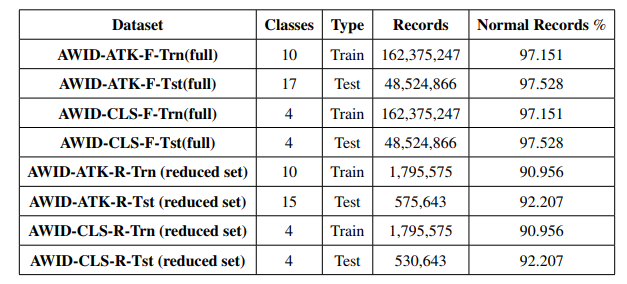
\includegraphics[width=0.49\textwidth]{Figures/AWID_Class Distribution.PNG}
%\caption{Aegean Wi-Fi Intrusion Dataset (AWID) record distribution}

 %  \end{figure}
 %   \begin{figure}
 %    \centering
%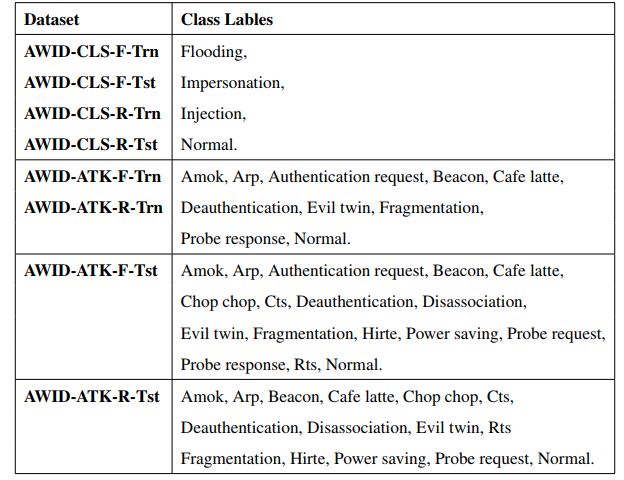
\includegraphics[width=0.49\textwidth]{Figures/class_dist.PNG}
%\caption{Aegean Wi-Fi Intrusion Dataset (AWID) class distribution}

%   \end{figure}




% Thesis: https://pdfs.semanticscholar.org/8748/34ea68ba0e99b48937ce61af2759d9862e33.pdf

% DtypeWarning: Columns (37,38,39,40,41,42,43,44,45,47,48,49,50,51,52,53,54,55,56,57,58,59,60,61,62,74,88) have mixed types.


 We observed a use of Artificial neural networks (ANN) with enhanced resilient back-propagation for the design  in ref \cite{Naoum2012}. In \cite{Gao2014}, the work used an unsupervised greedy learning algorithm to learn similarity representations over the nonlinear and high-dimensional data in NSL-KDD dataset. The results show that four-hidden-layer Restricted Boltzmann machines can produce the higher accuracy in comparison with SVM and ANN.  In recent years, deep Neural Networks with three or more hidden layers support higher generalization capability in comparison to ANN \cite{Kaynar2017}. The model is fed inputs, inputs get multiplied by weights and the passed into an activation function. The model uses backpropagation to adjust weights and increase accuracy. To be noted, most of the intrusion detection algorithms in the literature were found to be developed on on the NSL-KDD dataset, which is based on the KDD Cup 99 dataset \cite{NSLKDD}.

%In \cite{Li2015}, a deep belief network for malicious code detection method was reported that included an autoencoder based dimensionality reduction technique. An accelerated deep architecture was introduced in Potluri et al. \cite{potluri2016} to identify the abnormalities in the network data. They evaluated the performance of the model training related to different processor types and number of cores. Li et al. \cite{Li2017} presented an intrusion detection method using convolutional neural networks which adopts a novel representation learning method of graphic conversion. However, the model accuracy ranged from 79\% to 81.57\% which did not justify the increased latency added by the representation learning of the feature space. In reference \cite{Vinay2017}, Vinaykumar et al. reported various convolutional and recurrent neural network architectures for IDS implementation, however their results for under-represented remote to local (R2L) and user to root (U2R) attacks were very low. Shone et al.\cite{Shone2018} reported a stacked non-symmetric deep auto-encoders with random forest classifier achieved an overall accuracy of 85.42\%, with very poor performance on the R2L and U2R intrusion categories. A stacked autoencoder based implementation of NIDS by Farahnakian et al.  \cite{Farah2018} produced high accuracy (94.71\%) and high detection rate (94.53\%), however, these models could still be improved. 
In 2015, the Aegean Wi-Fi Intrusion Dataset
(AWID) \cite{AWID} was released as a comprehensive 802.11 network dataset that was derived from real Wi-Fi traffic traces. In the initial research with AWID, Kolias et al \cite{AWID_main}  applied several conventional supervised machine learning algorithms to perform the attack classification on the AWID dataset for accurate wireless network intrusion detection. They carried out manual feature selections and the top 20 features were chosen to train 8 classifiers. The overall accuracy of their classifiers ranges from 89.43\% to 96.2\%
 There are many proposed approaches in literature such as majority voting \cite{alotaibi2016majority}, multi-agent models \cite{kaleem2016cognitive}, deep learning models \cite{aminanto2018deep,abdulhammed2018machine}  where autoencoderbased models were used for detecting the attack categories in AWID dataset. However, Aminanto et al. \cite{aminanto2018deep} proposed an algorithm that can detect an impersonation attack by reducing the features dimensionalities and adopting stacked autoencoder at the fifinal stage. However, they did not include flooding and injection attacks in consideration. 
The findings from our literature review have shown that despite the high detection accuracy being achieved, with most researchers still experimenting on combining various algorithms (e.g. training, optimisation, activation and classification) and layering approaches to produce the most accurate and efficient solution for a specific dataset. A further accuracy-wise comparison of the methods in term of learning approach and accuracy is presented in \tab{table:performance_comparison}.

For this research, we focused on exploring low latency models while maintaining high accuracy by proposing a hybrid deep neural network that includes an unsupervised pre-training using autoencoders to make the model more adaptive to the changes in the network traffic. We then used a dedicated supervised dense neural network structure for the final classification. While designing, we made sure the memory or processing power to train and execute machine learning models are within the capability of the routers processing power. We hence believe the model and work presented in this paper will serve towards the real time and low latency implementation of the NIDS models.

\section{Data Pre-processing and Implementation of the model}
In this section, we discuss on the technical details of our proposed deep learning based approach to increase the performance accuracy of the Aegean WiFi Intrusion Dataset (AWID). AWID is a publicly available collection of sets of data in an easily distributed format, which contain real traces of both normal and intrusive 802.11 WLAN\cite{AWID_main}. Each record in the dataset is represented as a vector of 156 attributes, with the last attribute being class. Each record is composed mainly by MAC layer information.
%Such attributes include: Source Address (wlan\_sa), Destination Address (wlan\_da), Initialization Vector (wlan\_wep\_iv), the ESSID (wlan\_mgt\_ssid) and others. Additionally, all Radiotap information such as the Signal Strength (radiotap\_dbm\_antsignal),as well as general frame information such as Packet Number (frame\_number) are included in each record.
All attributes in the dataset have numeric or nominal values and the scales of the attributes on the dataset are heavily imbalanced. For example, a typical MAC address corresponds to an integer value of 82468889197, while a typical value of signal strength field is −33. Hence different types of encoding or normalization step would be necessary prior to applying any kind of machine learning algorithm to the dataset.
There are two types of AWID dataset. The first type named “CLS”, has four target classes, whereas the second, named “ATK”, has 16 target classes. The 16 classes of the “ATK” dataset belong to the four attack categories in the “CLS” dataset.

For this research we have used the Reduced four class dataset (AWID-CLS-R-Trn, AWID-CLS-R-Tst) scenario with three attack classes (flooding, impersonation and injection) and one normal category for training and classification purposes. Further description on the features extracted in the dataset can be found in ref \cite{AWID_main, AWID}. The data contained in the AWID dataset are diverse in value, discrete, continuous, and symbolic, with a flexible value range. These data characteristics could make it difficult for the classifiers to learn the underlying patterns correctly.

\subsection{Data Pre-processing}

In training and the test dataset there is a total number of 2,371,281 instances labelled data records. We used 20\% of the entire dataset as test set, the remaining 80\% of the data was used for training and validation purpose. As mentioned previously, the dataset contains different features with different value ranges. We conducted a detailed statistical analysis to monitor feature-wise values for minimum, maximum and standard deviation. We have replaced missing values with zeroes, dropped out the features with duplicate information and the columns with constants values as they contain no class-wise distinction. This analysis resulted in 36 unique features that was then fed to the autoencoded learning layer of our proposed model. We have also applied log encoding on the large numerical features such as source bytes, destination bytes and duration to avoid any kind of biasing on the training due to their large values. There were a number of features that needed conversion to 16-bit integer form  before they could be fed to the model.  As technology becomes more and more integrated, security of these systems over wireless networks is becoming more important. Over the years we have seen an increase in hacks in banking systems, healthcare systems and many Internet of Things (IoT) devices. We then performed a \emph{standard scaler} function as a normalization operation on the feature vectors of the dataset. Finally, the output labels are \emph{one hot encoded}. As a result, the total number of input dimension is 36 after performing the above-mentioned steps and output dimension is four (three attack classes and 1 normal class).  
%The 36 features we used were "frame.time_delta","frame.time_delta_displayed","frame.time_relative","frame.len","frame.cap_len", "radiotap.length", "radiotap.present.tsft", "radiotap.present.flags","radiotap.present.channel", "radiotap.present.dbm_antsignal","radiotap.present.antenna","radiotap.present.rxflags", "radiotap.datarate","wlan.fc.type_subtype", "wlan.fc.type", "wlan.fc.subtype", "wlan.fc.ds", "wlan.fc.frag", "wlan.fc.retry", "wlan.fc.pwrmgt", "wlan.fc.moredata", "wlan.fc.protected", "wlan_mgt.fixed.capabilities.cfpoll.ap", "wlan_mgt.fixed.listen_ival", "wlan_mgt.fixed.status_code" "wlan_mgt.fixed.timestamp", "wlan_mgt.fixed.aid", "wlan_mgt.fixed.reason_code", "wlan_mgt.fixed.auth_seq", "wlan_mgt.fixed.chanwidth", "wlan_mgt.tim.bmapctl.offset", "wlan_mgt.country_info.environment", "wlan_mgt.rsn.capabilities.ptksa_replay_counter", "wlan_mgt.rsn.capabilities.gtksa_replay_counter", "wlan.qos.ack", and "class".

% \FloatBarrier

%%%%%%%%%%%%%%%%%%%%%%%%%%%%%%%%%%%%%%%%%%%%%%%%%%%%%%%%%%%%%%%%%%%%

\subsection{Proposed Model}
 
 
\fig{fig:Architecture} illustrates the work flow and the proposed deep model architecture for the intrusion detection system. Similar to most existing deep learning research, our proposed classification model was implemented using python keras library \cite{keras} with TensorFlow back end. All of our evaluations were performed on a Windows machine with an Intel Xeon 3.60GHz processor, 32 GB RAM and an NVIDIA GTX 1050 GPU. 

We considered the following factors during our implementation of the IDS for the wireless realm:
(a) The system should provide extremely low on false positive (FP) alerts due to the large volume of data, a FP rate of 1\% may generate a great number of false alerts on daily basis.
(b) It should be highly adaptive to drastic network behavioral changes due to new events or natural changes in equipment, network behavior that once seemed normal may start looking suspicious. The system should also be able to detect novel attacks—as wireless technologies change, new vulnerabilities should be added in the system on a regular basis.

We employed two main functional stages in our proposed model. An auto-encoder based unsupervised pre-training layer and a supervised dense neural network for classification of the attack types for the NIDS. We describe our intuition for using these components in the system development in the coming subsections.

 \begin{figure}
      \centering
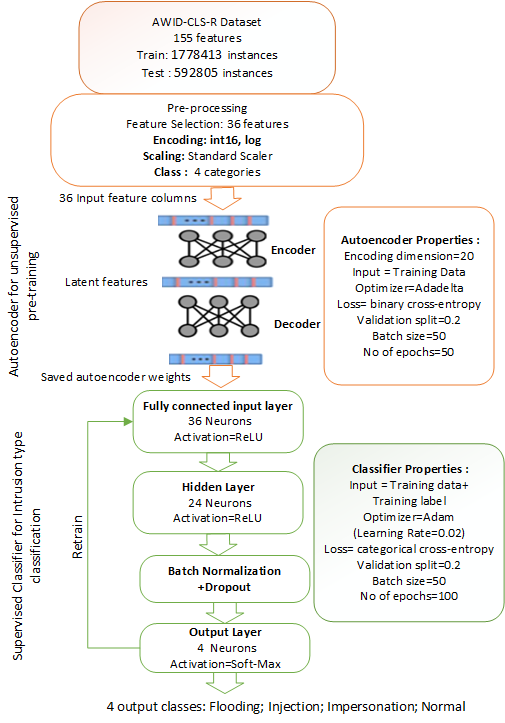
\includegraphics[width=0.48\textwidth]{Figures/NIDS_Autoencoder_Architecture.png}
\caption{Workflow and architecture of the proposed  autoencoded dense neural network}
      \label{fig:Architecture}
    \end{figure}
%
 %\begin{figure}
%      \centering
%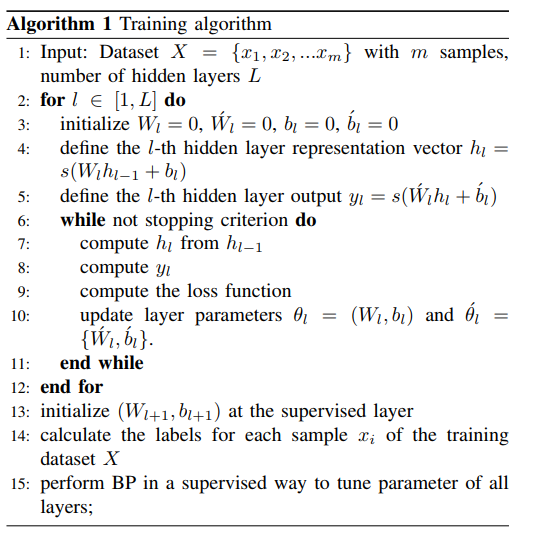
\includegraphics[width=0.49\textwidth]{Figures/Algorithm.PNG}
%\caption{Algorithm}
%\label{fig:Algorithm}
%    \end{figure}



%%%%%%%%%%%%%%%%%%%%%%%%%%%%%%%%%%%%%%%%%%%%%%%%%%%%%%%%%%%%%%%%%%
   
\subsubsection{ Unsupervised pre-training with Autoencoder}
An autoencoder is a type of artificial neural network used to learn efficient data representation in an unsupervised manner. In our proposed model, we have employed an autoencoder with an encoding and a decoding layer  that has been trained to minimize the reconstruction error. This incorporated prior knowledge from the training set to effectively learn from the data itself and provide good performance. Such pre-training allow both the data for the current task and for previous related tasks to self-organize the learning system to build the learning system in a data driven fashion. We have fed the autoencoder with the features from the training dataset without labels (unsupervised). A set of compressed and robust feature is built at the end of this step. The encoder part of the autoencoder aims to compress input data into a low-dimensional
representation, and there is a decoder part that reconstructs input data based on the low-dimension representation generated by the encoder.

For a given training dataset $X = \{x_1, x_2, ..., x_m\}$ with
m samples or instances, where $x_n$ is an n-dimensional feature vector, the
encoder maps the input vector $x_n$ to a hidden representation
vector $h_n$ through a deterministic mapping $f_{\theta}$ as given in \equ{equ:encoder}
\begin{equation}
\label{equ:encoder}
h_n = f_{\theta}(x_n) = \sigma(W x_{n} + b)
\end{equation}
where W is a $p \times p$, p is the number of hidden units, b is a bias vector, $\theta$ is the mapping parameter set $\theta = \{W, b\}$. $\sigma$ is sigmoid activation function.

The decoder maps back the resulting hidden representation
$h_n$ to a reconstructed p-dimensional vector $y_n$ in input space.
\begin{equation}
\label{equ:encoder}
y_i = g_{\theta}(h_n) = \sigma(W h_{n} + b)
\end{equation}
The goal of training the autoencoder is to minimize the
difference between input and output. Therefore, a error function
is calculated by the following equation:
\begin{equation} E(x,y)= {\frac{1}{m}}\norm{\sum\nolimits_{i=1}^{m}(x_{n}-y_{n})}^{2} \end{equation}
The main objective is to find the optimal parameters to minimize the difference between input and reconstructed output over the whole training set (m).

\subsubsection{ Supervised Classification with DNN}
After the autoencoder layer, a three layer dense neural network is employed of a  is trained by using the first autoencoder's output as inputs. This task sequence is retrained in a supervised manner with the class labels and the input feature given to the classifier. We have used a softmax activation layer as the output layer. The layer calculates the loss between the predicted values and the true values, and the weights in the network are adjusted according to the loss. 

The simple \emph{softmax} layer, which is placed at the final layer, can be defined as follows:
\begin{align}\label{eq3}
P\left( {c |x} \right) = {\text{argmax}}_{c \in C} \frac{{{ \exp }(x_{L - 1} W_{L} + b_{L} )}}{{\mathop \sum \nolimits_{k = 1}^{{N_{C} }} { \exp }(x_{L - 1} W_{k} )}},
\end{align}
where   $c$  is the number of classes,   $L$  is the last layer index, and $N_{C}$ is the total number of class types including normal network connection and intrusion.
After this stage, all layers are fine-tuned through back-propagation in a supervised way. In the test phase, the softmax layer outputs the probability of the predicted categories. The proposed algorithm is summarized here in Algorithm I.

%%%%%%%%%%%%%%%%%%%%%%%%%%%%%%%%%%%%%%%%%%%%%%%%%%%%%%%%%%%%%%%%%%

 \begin{figure}
      \centering
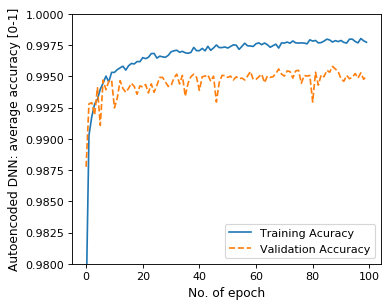
\includegraphics[width=0.30\textwidth]{Figures/Autoencode_DNN.png}
\caption{ Training and validation set accuracy over increasing number of epochs( training iterations) }
      \label{fig:accuracy}
    \end{figure}
%%%%%%%%%%%%%%%%%%%%

%%%%%%%%%%%%%%%%%%%%%%%%%%%%%%%%%%%%%%%%%%%%%%%%%%%%%%%%%%%%%%%%%%%%%


\begin{algorithm}[h]\label{algorithm}
\small 
\KwIn{ Taining dataset $X = \{x_1, x_2, ..., x_m\}$, Number of layers $L$}

\nl for $l \in\mathcal [1, L]$ do\;
\nl \ Initialize $ W_l = 0, W´_l = 0, b_l = 0, b'_{l} = 0$\;
 {Encoding layer}\;
\nl \ Calculate encoding or hidden representation using equation(1)\;
\ \  \ \ \  $ h_{l} = s(W_{l}x_{l−1} + b_{l})$\;
{Decoding layer}\;
\nl\ while not loss==stopping criteria do\;
\nl \ \ Compute $y_{l}$ using equation (2)\;
\nl \ \ Compute the loss function: binary cross-entropy\;
\nl\ \ Update layer parameters  $\theta = \{W, b\}$\;
\nl \ end while\;
\nl end for\;
{Classifier:Dense neural network, Soft-max activation at the output layer}\;
\nl Initialize $(W_{l+1}, b_{l+1})$ at the supervised layer\;
\nl {Calculate the labels for each sample $x_n$ of the training dataset $X$}\;
\nl Apply batch normalization and dropout for speeding up the calculation\;
\nl {Perform back-propagation in a supervised manner to tune parameters of all layers, loss function categorical cross-entropy\;}

\nl  end\;
\KwOut{Class labels}
    {\caption{\bf Auto-encoded DNN training algorithm} \label{Algorithm}
    }
\end{algorithm}

%\FloatBarrier
\subsubsection{ Speeding up the training phase}
\fig{fig:accuracy} plots the network training process for 100 iterations. During training, we have used additional techniques such as dropout and batch normalization to avoid over fitting and also to speedup the training process. The proposed algorithm   achieves approximately 99\% accuracy for the training set in 20 iterations which is four times faster than the generic model with no dropout and batch normalization employed. We used a five-fold cross-validation using 20\% of the training data as the validation data set. Potentially this allows a reduction in the training epochs required, and will be of vital importance for developing low-latency models and training future networks with bigger data sets.

\section{Model Evaluation} \label{sec:evaluation}
To prove the efficacy of our designed model, our aim is to show that the intrusion detection system will maximize attack prediction accuracy  while minimizing any falsely categorized values.
%%%%%%%%%%%%%%%%%% RESULTS %%%%%%%%%%%%%%%%%%
\subsection{Confusion Matrix}

We presented the confusion matrix plot  in \fig{fig:confusionmatrix}, for our model when evaluated with the test data set. The rows correspond to the predicted class (Output Class) and the columns correspond to the true class (Target Class). If True Positive ($T_P$) is the number of attacks classified
rightly as attack; True Negative ($T_N$) is the number of normal
events rightly classified normal; False Positive ($F_P$) is the
number of normal events misclassified as attacks and False
Negative ($F_N$) is the number of attacks misclassified as
normal, the diagonal cells in the confusion matrix correspond to observations that are correctly classified ($T_P$ and $T_N$'s). The off-diagonal cells correspond to incorrectly classified observations ($F_P$ and $F_N$'s). Both the number of observations and the percentage of the total number of observations are shown in each cell.
%%%%%%%%%%%%%%%%%%%%%%%%%%%%%%%%%%%%%%%%%%%%%%%%%%%%%%%%%%%%%%%%%%%%%
 \begin{figure}
      \centering
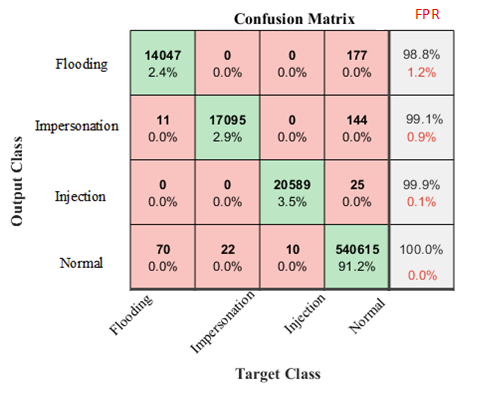
\includegraphics[width=0.45\textwidth]{Figures/cm.png}
\caption{Confusion matrix of the test dataset}
      \label{fig:confusionmatrix}
    \end{figure}
  %   \begin{figure}
 %     \centering
%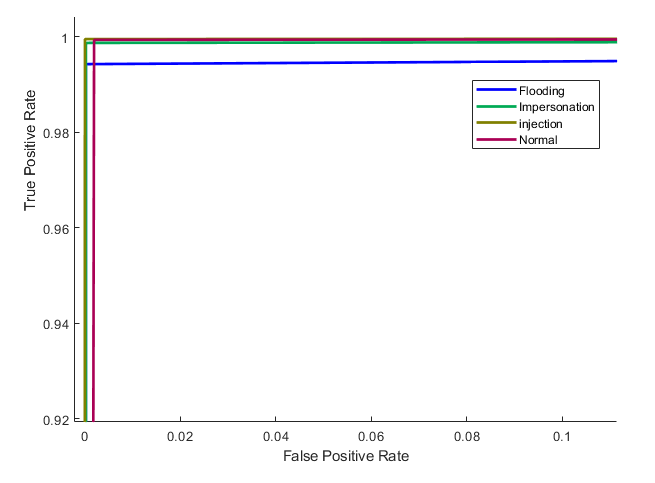
\includegraphics[width=0.39\textwidth]{Figures/RoC_curve.png}
%\caption{Receiver operating characteristics for different classes}
%      \label{fig:RoC}
    %\end{figure}
   

The column on the far right of the plot shows the percentages of all the examples predicted to belong to each class that are correctly and incorrectly classified. These values are often called the precision and false discovery rate respectively. To be noted, we have utilized builtin Matlab function \emph{plotconfusion(true class, predicted class)} for generating  \fig{fig:confusionmatrix}. Both true class and predicted class variables were one-hot encoded and imported from the python interface as .mat file for plotting purposes.

We can also define accuracy, recall, precision and F1 values of a model  using the following equations:

\begin{itemize}
\item {Accuracy: It is an indicator of the total number of correct predictions provided by the model and defined as follows:

\begin{align}
\text{Accuracy} =\frac{T_P+T_N}{T_P+T_N+F_P+F_N}.
\end{align}
}
\item {Recall, precision and F measure: Three of the most commonly used performance measures with F measure being the harmonic mean of recall and precision measures are defined as follows:
\begin{align}
\text{Recall or True positive rate} =\frac{T_P}{T_P+F_N}.
\end{align}
\begin{align}
\text{Precision} =\frac{T_P}{T_P+F_P}.
\end{align}}
\begin{align}
{\text{F \ Measure}} =\frac{2*{\text{Precision}}*{\text{Recall}}}{\text{Precision+Recall}}
\end{align}

 
%\item {F1 Score:It is the harmonic mean of precision and recall and defined as follows:
%\begin{align}
%{\text{F1 \ Score}} =\frac{2*{\text{Precision}}*{\text{Recall}}}{\text{Precision+Recall}}.
%\end{align}}
\end{itemize}
%\fig{fig:RoC} showed the class-wise receiver operating characteristic (ROC) for our proposed model. The model produced highly accurate predictions for the classes of the designed NIDS.
We obtained a true positive rate (TPR) of above 99\% for all the attack categories and normal connection.  For flooding attacks, there were only 1.2\% (177 wrong predictions out of 14k instances) false predictions made by the model. For the injection and impersonation type attacks, its even lower as 0.1\% and 0.9\% respectively (also presented in the rightmost column in \fig{fig:confusionmatrix}). For the normal connection classification there were only 92 instances out of 540k test cases that was misclassified by the model.

     \begin{table*}
     \centering
    \caption{Comparison of the proposed method with other machine learning techniques for AWID four-class intrusion detection}   \label{table:performance_comparison}
  \begin{tabularx}{0.99\textwidth}{X  cc c c  cc}
    \toprule
    Learning method & Dataset  &  Flooding & Injection& Impersonation&Normal& Overall Accuracy (\%) \\
    \otoprule
   J48 (20 features) \cite{AWID_main}&AWID-CLS-R&99.83&100&70.55&96.14&96.2 
\\
     Random Forest(20 features) \cite{AWID_main}& AWID-CLS-R  &99.97&99.42&99.92&95.44& 95.6 \\ 
    
  Majority Voting (154 features)  \cite{alotaibi2016majority}& AWID-CLS-R&100&100&100&96.15  &96.32   \\
    \hline
    
    Multi-Layer Perceptron (32/7/5 features)   \cite{abdulhammed2018machine}&AWID-ATK-R &-&-&- &-& 96.21 \\
    3-hidden-layer deep architecture\cite{thing2017ieee}&AWID-ATK-R &34.15&82.58&0& 99.93&95.02 \\
    Neural Network (154/6 features)\cite{kaleem2016cognitive}&AWID-CLS-R  &-&-&-&-& 99.3 \\
   Stacked Autoencoder (35 features)\cite{aminanto2018deep}&AWID-CLS-R  &-&-&-&-& 99.88 \\
    
 \bf{ Proposed Autoencoded DNN (36 features)} &  AWID-CLS-R  &99.42&99.87 &99.9&99.93&99.9 \\
    \bottomrule
  \end{tabularx}
\end{table*}

%\FloatBarrier


\subsection{Comparison with other approaches}

 There were several neural network and deep learning based methods presented in \cite{kaleem2016cognitive, aminanto2017improving,aminanto2018deep,thing2017ieee}, with variable accuracy for the under-represented attack classes. Our results showed an excellent performance with an overall detection accuracy of  99.9\%. \tab{table:performance_comparison} summarizes the class-wise true positive rate (TPR) and overall accuracy of our proposed model with some concurrent deep learning methods, our work outperforms previous related work in terms of number efficient selection of features and accuracy. 
   

 
%%%%%%%%%%%%%%%%%% CONCLUSIONS %%%%%%%%%%%%%%%%%%

\section{Conclusions} \label{sec:conclusions}
 Cyber threats have become a prime concern for information security. NIDS is one of the security mechanisms used to guard these applications against attacks. In this research, we have applied a deep network intrusion detection model and evaluated the algorithm with the benchmark AIWD dataset. Currently, the algorithm is trained offline on high performance computer. Our  results  showed  an  excellent  performance  with  an overall  detection  accuracy  of  99.8\%  for  Flooding or DoS, Injection and  Impersonation type  of attacks. We also presented a comparison with recent approaches used in literature which showed a substantial improvement in terms of accuracy and latency with proposed autoencoded DNN. In future, we will provide extensions or modifications of the proposed algorithm for larger attack types , mobile and IoT security platforms as suggested in ref \cite{abdulhammed2018machine} using intelligent agents  such as soft computing and advanced unsupervised clustering algorithms. Because of the availability of deep learning libraries in python such as Keras and TensorFlow Lite, on-device machine learning inference is now possible with low latency. Hence, future models will cover a broader range of attacks, respond in real time and update itself over time. Future extension of this work will be to improve the detection accuracy and to reduce the rate of false negatives and false positives in attack detection to improve the systems performance.
 \FloatBarrier

%%%%%%%%%%%%%%%%%% REFERENCES %%%%%%%%%%%%%%%%%%
\renewcommand*{\bibfont}{\small}
\printbibliography


\end{document}
